\section{Processos de Software}

Engenharia de Software pode ser definida como:
\begin{citacao}[english]
1. the systematic application of scientific and technological knowledge, methods, and experience to the design,
implementation, testing, and documentation of software [...]  2. the application
of a systematic, disciplined, quantifiable approach to the development, operation,
and maintenance of software; that is, the application of engineering to software \cite{IEEE2010}.
\end{citacao}

A engenharia de software deve ter foco na qualidade, que apoia as outras camadas
dessa tecnologia, que são as camadas de processo, métodos e ferramentas \autoref{fig:desen_engsoft}.
A camada de processo define um conjunto de atividades ou um arcabouço que tem
como finalidade garantir a efetiva utilização da tecnologia engenharia de software, que dessa forma
leva à produção de um software. Os detalhes de como fazer o software pertencem
a camada de métodos. Os métodos da engenharia de software incluem tarefas de planejamento
e estimativa de software, análise de requisitos, modelagem de projeto, codificação,
testes e manutenção. As ferramentas de engenharia de software auxiliam as camadas de
processo e métodos, com ferramentas automatizadas, que por sua vez, quando integradas,
é estabelecido um suporte ao desenvolvimento de software chamado CASE -
\textit{Computer Aided Software Engineering} \cite{Pressman2009, Sommerville2006}.

\begin{figure}[b]
  \centering
  \caption{Engenharia de Software - uma tecnologia em camadas}
  
\includegraphics[scale=0.3]{imagens/desenv_engsoft2}
  \label{fig:desen_engsoft}
  \fonte{\cite{Pressman2009}}
\end{figure}

Entre o conjunto de atividades definidas pela camada de processo, quatro são
fundamentais, a saber, especificação de software, projeto e implementação de
software, validação de software e evolução de software. Especificação de software
ou engenharia de requisitos é uma fase importante e crítica do processo de engenharia
de software. Importante porque é uma análise de requisitos bem feita que possibilitará
atendar as demandas dos usuários. Crítica porque um sistema mal especificado, pode até ser
bem projetado e construído, mas não vai atender as necessidades dos usuários.
Em seguida, na fase de projeto e implementação os requisitos são projetados e programados,
tendo como resultado um sistema executável. Depois, o software deve ser verificado
para mostrar que atende às demandas dos usuários (validação do software). Finalmente,
na fase de evolução de software, o mesmo é modificado devido às mudanças
de requisitos e às necessidades dos usuários.

% Quanto ao modelos de engenharia de software temos os modelos prescritivos e os ágeis.
% Os modelos prescritivos definem um conjunto de atividades explícitas para serem
% desenvolvidos no processo de engenharia de software. O Processo Unificado de desenvolvimento
% tem o maior destaque e reconhencimento dentre os modelos prescritivos.
%
% \subsection{Processo Unificado}
% O Processo Unificado define quatro atividades no processo de desenvolvimento de software.
% As fases são descritas como:
%
% \begin{description}
%   \item [{Concepção:}] Por meio da comunicação com os clientes, um conjunto
%   preliminar de casos de uso UML e da arquitetura do sistema é elaborada.
%   \item [{Elaboração:}] Nessa fase, os casos de uso UML são expandidos e
%   refinados, bem como a definição da arquitetura do sistema. Ao final
%   dessa fase, um conjunto de casos de uso UML descrevem os requisitos
%   dos sistema. Uma descrição da arquitetura do sistema e um plano de
%   desenvolvimento do software também são esperados.
%   \item [{Construção:}] Os casos de uso UML desenvolvidos na fase de elaboração
%   são então desenvolvidos e testados. O software deve estar funcionando
%   e documentado na conclusão dessa fase.
%   \item [{Transição:}] transferência do software aos usuários finais.
% \end{description}
%
% Fluxos de trabalhos ou \emph{workflows} ocorrem durante todas as
% fases no processo de desenvolvimento. São seis \emph{workflows} principais
% e três de apoio:
% \begin{enumerate}
%   \item \emph{Modelagem de negócios}: processos de negócios modelados por
%   casos de uso.
%   \item \emph{Requisitos}: atores são idenficados e casos de uso são desenvolvidos.
%   \item \emph{Análise e projeto: }vários modelos são desenvolvidos como de
%   arquitetura e componentes.
%   \item \emph{Implementação: }componentes são implementados.
%   \item \emph{Teste: }processo iterativo em conjunto com a implementação.
%   \item \emph{Implantação: }software é distribuído aos usuários finais.
%   \item \emph{Gerenciamento de configuração e mudança: }apoio as mudanças
%   do sistema.
%   \item \emph{Gerenciamento de projeto: }apoio de desenvolvimento do sistema.
%   \item \emph{Meio ambiente: }apoio a equipe de desenvolvimento com ferramentas.
% \end{enumerate}
%
\subsection{Métodos Ágeis}

Contrapondo-se aos modelos prescritivos em que propoem especificar por completo
os requisitos do sistema e só então projetar, construir e testar o sistema, surgiu
os métodos ágeis, que têm como filosofia o manifesto ágil. Esse manifesto afirma:

\begin{citacao}
  Estamos descrobrindo melhores maneiras de desenvolver softwares, fazendo-o e ajudando
  outros a fazê-lo. Através dessse trabalho, valorizamos mais:\\\\
  \begin{minipage}{15cm}
    \begin{itemize}
      \item Indivíduos e interações do que processos e ferramentas
      \item Software em funcionamento do que documentação abrangente
      \item Colaboração do cliente do que negociação de contrato
      \item Resposta a mudanças do que seguir um plano
    \end{itemize}
  \end{minipage}\\\\
  Ou seja, embora itens à direita sejam importantes, valorizamos mais os que estão à esquerda.
\end{citacao}

Abordagens ágeis incluem \textit{Extreme Programming} e o \textit{Scrum}. Eles propõem diferentes processos
para que tenha-se um desenvolvimento e entrega incremental do sistema, tendo em comum princípios
baseados no manifesto ágil.

\section{Metodologias e Ferramentas}

A metodologia escolhida nesse projeto levou em consideração as necessidades de um trabalho de
conclusão de curso no curto prazo e os recursos limitados. Dessa forma, uma abordagem baseada em metodologias ágeis foi utilizada para %modelagem, documentação e codificação do software.
especificação, projeto e implementação do software. Nesse sentido, por exemplo,
na fase elicitação de requisitos não procurou-se a completa definição dos requisitos do software e ela nem foi
uma fase, a elaboração contínua dos requisitos fez parte do projeto de desenvolvimento como um todo.

% Práticas fundamentais implicam em aplicar os artefatos de modelagem corretos para cada situação, modelando o problema de forma incremental – sem a necessidade de criação de uma modelagem completa, irreal e fadada a ser, necessariamente, abandonada ou modificada posteriormente. Acredita-se ainda que os stakeholders do processo possuam o conhecimento sobre o que querem e podem prover tal conhecimento através de participação ativa, solicitada pelos modeladores.
%

\subsection{Objetivos específicos}

Para cada objetivo específico deste trabalho, as seguintes técnicas e ferramentas foram utilizadas:

\subsubsection{Realizar levantamento de requisitos sobre os sistemas de resposta em sala de aula}

A elicitação inicial de alto nível dos requisitos do sistema utilizou a análise de competidores que
consistiu basicamente em buscar em alguns sistemas de resposta existentes, referências positivas e
negativas para definição do modelo a ser proposto.

\subsubsection{Especificar e implementar uma aplicação web para o professor administrar as questões e gerar relatórios}

Com os requistos da primeira etapa, tivemos os requisitos inicias para a aplicação desktop do professor.
O \textit{Ionic} também foi utilizado na aplicação desktop do professor.

\subsubsection{Especificar e implementar uma aplicação para dispositivos móveis, que será utilizado como {\clickers}}

Com os requisitos da primeira etapa, tivemos os requisitos inicias para a aplicação móvel.
A linguagem de programação usada na fase de implementação do aplicativo foi JavaScript, tendo como auxílio o \textit{framework} \textit{Ionic}.

O \textit{Ionic} é um \textit{framework} de código aberto para o desenvolvimento de aplicativos híbridos e desktop utilizando
tecnologias web como HTML, CSS e JavaScript otimizados para dispositivos móveis, com código fonte sobre a licença MIT.

\subsubsection{Especificar e implementar um sistema servidor, para receber e
    enviar dados para os os clientes: dispositivos móveis dos alunos e navegador
    web do professor}

O sistema servidor foi desenvolvido utilizando tecnologias como \textit{Node.js}, \textit{MongoDB}, e o \textit{framework} \textit{FeathersJS}.
Tais tecnologias foram utilizadas por permitir o fácil desenvolvimento de aplicações web de tempo real entre o servidor e os seus clientes.

A teoria mais aprofundada sobre os métodos e ferramentas citadas serão descritas nas próximas seções.

\section{Especificação}

A fase inicial do projeto foi a de planejamento para a definição inicial de alto nível dos
requisitos do sistema. Nessa etapa, utilizou-se a análise de competidores para elucidar
os requisitos que posteriormente foram descritos como histórias de usuário.

\subsection{Elicitação de Requisitos}

\subsection{Análise de competidores}

A análise de competidores é uma técnica oriunda engenharia da usabilidade
que consiste em avaliar produtos concorrentes em busca de pontos positivos e
negativos. Tal técnica é útil no levantamento de requisitos de um novo sistema,
identificação de pontos fortes e fracos os produtos, reutilização de design, dentre outros.

Avaliar produtos concorrentes é valioso, porque oferece a oportunidade de novos
produtos evitarem problemas existentes dos competidores, explorar os pontos
fracos, além da reutilização dos pontos positivos.

Nesse sentido, a análise de competidores foi utilizada neste trabalho para elicitar requisitos e boas práticas
de design de interfaces. % bem como evitar problemos já identificados pelos concorrentes
Os resultados obtidos foram utilizados no processo de desenvolvimento do software.

\subsubsection{\textit{Socrative}}

\textit{Socrative} é um sistema de resposta específico para usar em salas de aula. O sistema pode ser
acessado pelo site ou nos aplicativos para \textit{iOS} e \textit{Android}. No \textit{Socrative}, apenas o professor
precisa fazer um cadastro no site (questões demográficas são solicitadas). Existe uma versão
gratuita e paga do aplicativo.

Na conta do professor, é possível criar questionários de múltipla escolha, verdadeira e falso e
de questões abertas. Quando o professor cria uma conta, é gerado um código de identificação
para que os alunos possam entrar na sala virtual. Na interface do estudante, é necessário
colocar o código de identificação do professor.

\subsubsection{\textit{PollEverywhere}}

O \textit{PollEverywhere} é um sistema de resposta mais genérico, possibilitando fazer votações em
shows e apresentações diversas. Possibilita integração com ferramentas de apresentação
como o \textit{PowerPoint}. Outra característica é a possibilidade dos usuários votarem por SMS.
Além dos tipos de questões básicas, o \textit{PollEverywhere} permite criar nuvem de palavras e
questões com imagens clicáveis.

A conta do usuário é associado com uma URL, em que é usada para os participantes
da votação entrarem e votarem.

\subsubsection{\textit{TopHat}}

\textit{TopHat} é outra solução voltada para a educação, contando com seis tipos de questões.
Adicionalmente o \textit{TopHat} permite ao professor fazer a chamada dos estudantes, isso porque
o professor pode gerar um código aleatório no \textit{TopHat} para que os estudantes presentes
possam enviar o código e marcar presença. O produto também disponibiliza uma sala
de discussão e a possibilidade de criar slides dentro do aplicativo.

\begin{center}
\begin{table}
\begin{centering}
\begin{tabular}{>{\centering}m{4cm}||>{\centering}p{4cm}>{\centering}p{3.5cm}c}
\hline
\multicolumn{1}{>{\centering}m{3.5cm}}{Caraterística} & \textit{PollEverywhere} & \textit{TopHat} & \textit{Socrative}\tabularnewline
\hline
\hline
Open-Source & Não & Não & Não\tabularnewline
Integração com LMS & Blackboard & Excel & MasteryConnect\tabularnewline
Formatos & JSON, RSS, CSV & Não & Não\tabularnewline
Read-only API & Sim & Não & Não\tabularnewline
Integração com PowerPoint & Possibilita & Não & Não\tabularnewline
Métodos de votação & SMS, web & SMS, Web & Internet\tabularnewline
Tempo-real & Sim & Sim & Sim\tabularnewline
Acesso ao sistema & URL & Código de Acesso & Código de Acesso\tabularnewline
Tipos de questões & 5 & 7 & 3\tabularnewline
Mínimo de passos para votação & 2 & 3 & 4\tabularnewline
Anonimato & Possibilita & Possibilita & Possibilita\tabularnewline
Contagem regressiva & Possibilita & Possibilita & Não\tabularnewline
Download CSV & Possibilita & Não & Não\tabularnewline
Relatórios por estudante & Possibilita & Possibilita & Não\tabularnewline
\hline
\end{tabular}
\par\end{centering}

\caption{Análise de Competidores}
\end{table}

\par\end{center}

\subsection{Requisitos gerados a partir da análise de competidores}

A partir das informações coletadas na análise de competidores, foram
extraídos um conjunto de requisitos iniciais para o sistema. Os requisitos
funcionais gerados pela análise dos competidores foram então descritos como histórias de usuário.

\begin{description}
\item[Integração com sistemas LMS]: O sistema deve permitir integração com
sistemas LMS (preferencialmente Moodle);
\item[Todas as plataformas:] é muito importante que o sistema seja capaz
de funcionar em smartphones, tables e computadores independentemente
do sistema operacional.
\item[Questões abertas, verdadeiro/falso e de múltipla-escolha:] O sistema
deve fornecer pelo menos esses três tipos básico de questões;
\item[Modo de votação:] O sistema deve permitir votação anonima ou requisitar
a identificação;
\item[Customização das questões:] O sistema deve permitir inserção de equações
matemáticas (\LaTeX), imagens e texto como opção das questões;
\item[Controle da votação:] Opções básicas como ativar ou desativar a votação
e limpar uma votação em andamento;
\item[Controle de frequência:] o sistema gera um código aleatório ou uma
questão trivial, em que o professor pode solicitar que os estudantes
respondam, contando como controle de frequência. Os dados devem ser
facilmente exportados para CSV.
\item[Tempo-real:] No momento da votação, o professor pode escolher entre
apresentar o resultado em tempo-real, quando todos votarem, ou quando
determinado;
\item[Banco de questões:] As questões elaboradas pelo professor podem ser
armazenadas em um banco de questões que o sistema deve manter;
\item[Facilidade do uso e de criação de votação:] O sistema não deve oferecer
dificuldades de uso e de criação de questões;
\item[Código de acesso:] O sistema deve gerar um código de acesso único para
identificar o ambiente do professor, usado para que os alunos respondam.
\end{description}

\subsection{Histórias de Usuário}

A metodologia ágil de software, \textit{eXtreme Programming (XP)}, introduziu a
prática de expressar os requisitos de software na forma de \textit{histórias de usuário},
que são descricões informais do que o sistema deve fazer, evitando qualquer terminologia técnica.

As histórias de usuário (\autoref{fig:backlog}), formaram a lista de tarefas do projeto. Essa
lista de tarefas foi então priorizada, de forma que, por exemplo, desenvolver a arquitetura
que possibilita-se ao professor apresentar uma questão no quadro e habilitar para os alunos
responderem foi a primeira tarefa a ser desenvolvida. Por outro lado, a tarefa de permitir
categorizar as questões para permitir um agrupamento de questões teve uma priorização baixa.

\begin{figure}[!ht]
  \centering

  \subfloat{
    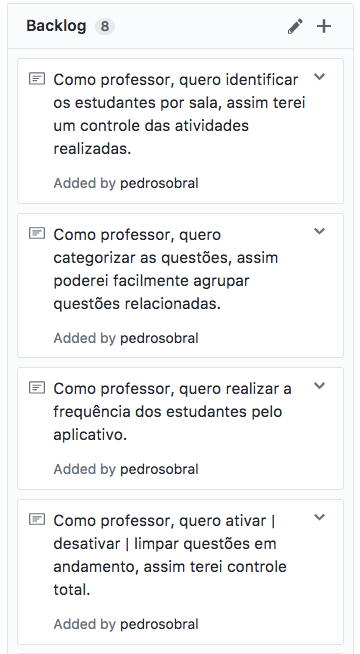
\includegraphics[scale=0.65,valign=t]{imagens/backlog1.png}
  }
  \subfloat{
    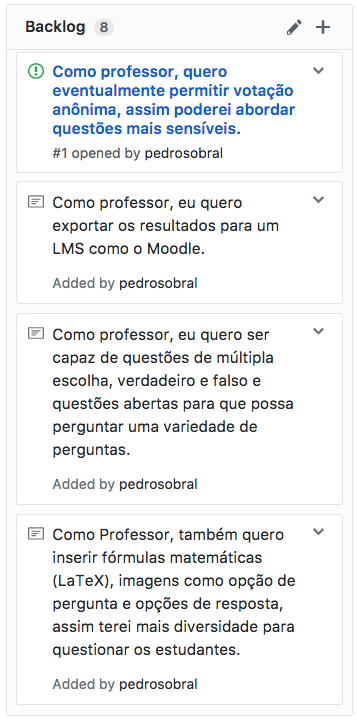
\includegraphics[scale=0.65,valign=t]{imagens/backlog2.png}
  }
  \caption{Requisitos iniciais para o sistema em forma de histórias de usuário}
  \label{fig:backlog}
\end{figure}


\section{Projeto e Implementação}

\subsection{Plataforma}

\begin{description}
  \item[JavaScript:] é uma linguagem de programação leve, interpretada e orientada a objetos com funções de primeira classe
  (funções no JavaScript podem ser passadas como argumento para outras funções, pode ser o valor retornado por outras funções e ainda
  podem ser atribuídas para variáveis).
  Ela é uma linguagem de scripting baseada em protótipos, multi-paradigma e dinâmica, suportando os estilos orientado a objetos, imperativo e funcional.
  Uma das implementações ou \textit{engine} mais populares de JavaScript é o V8 da Google que
  é utilizada pelo navegador Google Chrome e também pelo Opera.
  \item[Node.js:] é uma plataforma construída sobre o \textit{engine} V8 da Google
  para construir aplicações de rede rápidas e escaláveis. Node.js usa um modelo de I/O direcionada a
  evento não bloqueante que o torna leve e eficiente, ideal para aplicações em
  tempo real com troca intensa de dados através de dispositivos distribuídos.
  \item[MongoDB:] é um sistema de gerenciamento de banco de dados orientado à documentos.
  Ele é classificado como um banco de dados \textit{NoSQL}, ou seja, o mecanismo de
  armazenamento e recuperação é modelado de outras formas além da forma relacional. O MongoDB  usa o modelo de
  dados JSON para mapear as aplicações de forma simples e rápida.
\end{description}

\subsection{Arquitetura}

A \autoref{fig:arquitetura} exibe a arquitetura desenvolvida. O sistema
consiste dos clientes (aplicação professor e aplicativo dos alunos) que
fazem a requisição para o servidor desenvolvido na plataforma Node.js com o \textit{framework}
\textit{FeathersJS}. A comunicação entre os nós clientes e o servidor é por
meio do protocolo \textit{WebSocket}. O servidor faz a interface com o banco de
dados MongoDB.

\begin{figure}[!ht]
  \centering

  \caption{Arquitetura do sistema}
  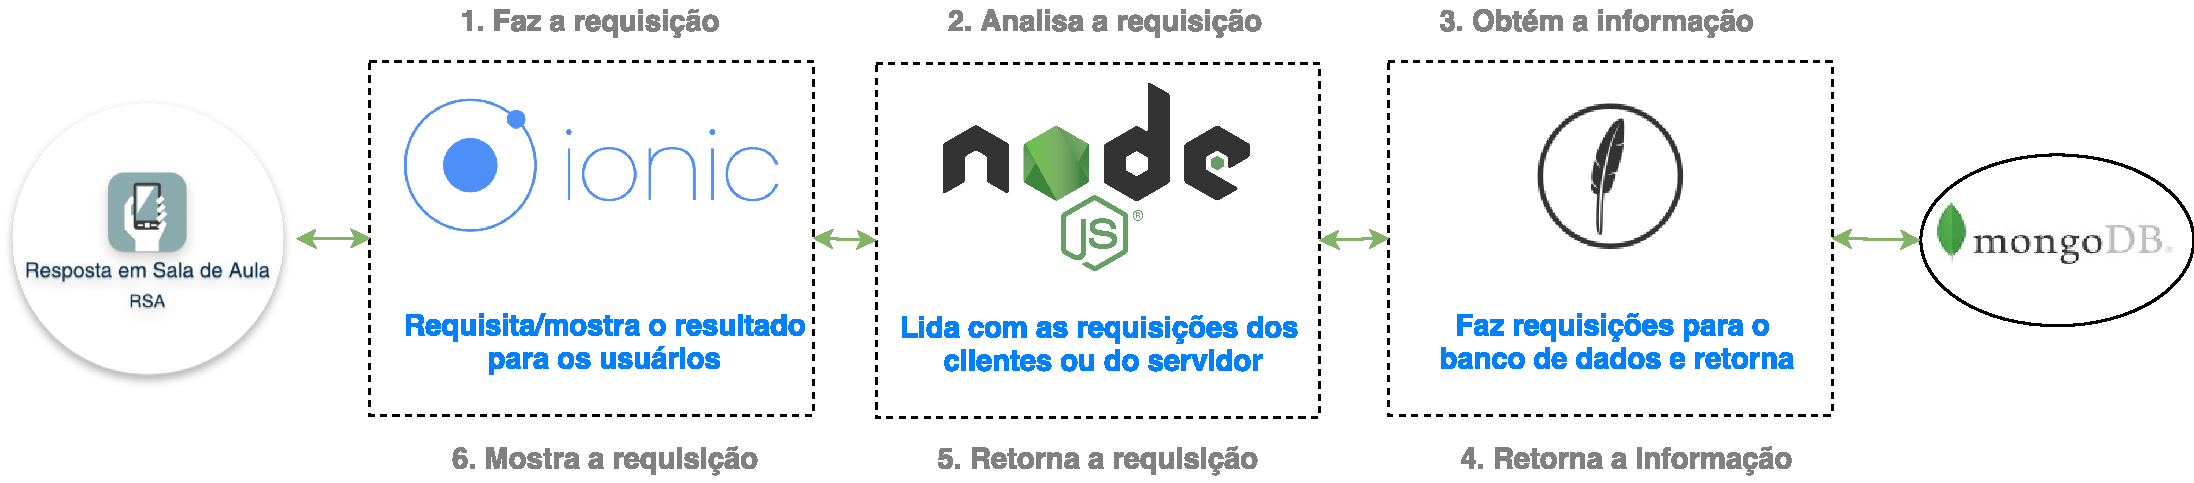
\includegraphics[scale=.45]{imagens/arquitetura.pdf}
  \label{fig:arquitetura}
  \doautor

\end{figure}

\subsection{\textit{WebSocket} para aplicações em tempo real}

\textit{WebSocket} é um protocolo que possibilita abrir um canal interativo de comunicação
entre o navegador e o servidor. Na verdade, esse canal é bidirecional (\textit{full-duplex})
que utiliza apenas um soquete TCP\nomenclature{TCP}{Transmission Control Protocol} \cite{websocket2016}.
A tecnologia \textit{WebSocket} foi usada para permitir votação e controle de frequência em tempo-real.

\subsection{Estrutura do Framework: \textit{Ionic}}

\textit{Ionic} é um \textit{framework open-source} para o desenvolvimento de aplicativos
híbridos utilizando tecnologias web como HTML\nomenclature{HTML}{HyperText Markup Language},
CSS\nomenclature{CSS}{Cascading Style Sheets} e JavaScript otimizadas
para dispositivos móveis, com código fonte sobre a licença MIT\nomenclature{MIT}{Massachusetts Institute of Technology} \cite{ionic2016}.
Uma das principais vantagens do desenvolvimento de aplicativos híbridos é que com
apenas um código base é possível criar aplicativos para várias plataformas como
\textit{iOS}, \textit{Android} e \textit{Windows} Phone, Desktop, que aliás foi uma das razões que fez o Moodle
usar o \textit{Ionic} como \textit{framework} para o desenvolvimento do \textit{Moodle Mobile 2} \cite{moodle2016}.

\subsubsection{Pages}

Um aplicativo desenvolvido no \textit{Ionic} é composto por um conjunto de pages ou páginas.
Cada página é composta por alguns arquivos. Um arquivo é responsável pelo
elemento visual da página, desenvolvido em HTML. Existe o arquivo de estilos da página,
desenvolvido em SCSS. O arquivo principal é o responsável por controlar a página, desenvolvido
em TypeScript.

As Figuras \ref{fig:hello_ionic_ts} e \ref{fig:hello_ionic_html} são um exemplo básico de
uma página de um aplicativo desenvolvido em \textit{Ionic}. O resultado dessa página é mostrado
na \autoref{fig:hello_world_ionic}. Observe que com apenas um código base, os elementos
visuais da página são diferentes dependendo da plataforma (\textit{iOS}, \textit{Android} e \textit{Windows}).

\begin{figure}[h]
\begin{lstlisting}[language=JavaScript]
  import { Component } from '@angular/core';

  @Component({
    selector: 'page-hello-ionic',
    templateUrl: 'hello-ionic.html'
  })
  export class HelloIonicPage {
    constructor() {}
  }
\end{lstlisting}
\caption{HelloIonicPage: classe responsável por exibir e controlar a página}
\label{fig:hello_ionic_ts}
\end{figure}

\begin{figure}[h]
\begin{lstlisting}[language=ionicHtml]
  <ion-header>
    <ion-navbar>
      <button ion-button menuToggle>
        <ion-icon name='menu'></ion-icon>
      </button>
      <ion-title>Hello Ionic</ion-title>
    </ion-navbar>
  </ion-header>

  <ion-content padding>

    <h3>Welcome to your first Ionic app!</h3>

    <p>
      This starter project is our way of helping you get a functional app running in record time.
    </p>
    <p>
      Follow along on the tutorial section of the Ionic docs!
    </p>
    <p>
      <button ion-button color='primary' menuToggle>Toggle Menu</button>
    </p>

  </ion-content>
\end{lstlisting}
\caption{HelloIonicPage: elementos visuais da página}
\label{fig:hello_ionic_html}
\end{figure}

\begin{figure}[h]
  \centering
  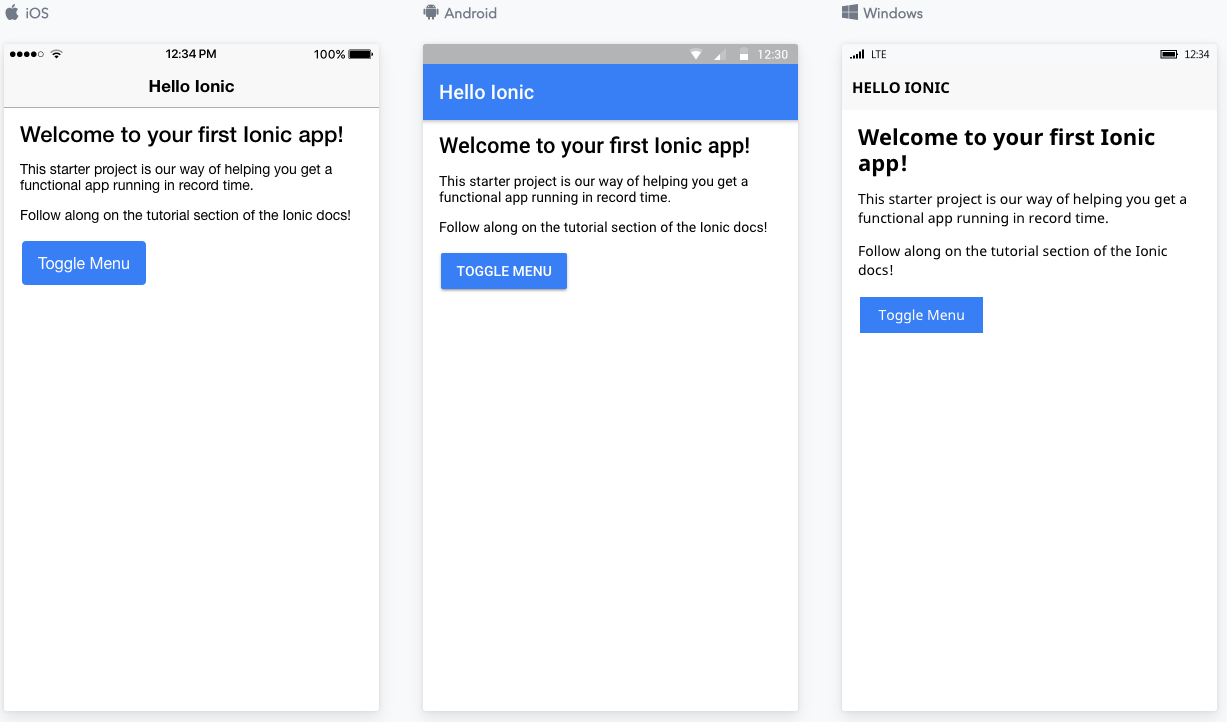
\includegraphics[scale=.4]{imagens/hello_world_ionic.png}
  \caption{Página em \textit{Ionic} resultado  das Figuras \ref{fig:hello_ionic_ts} e \ref{fig:hello_ionic_html}}
  \label{fig:hello_world_ionic}
\end{figure}

\subsubsection{Components}

Os elementos visuais e também o comportamento desses elementos em uma página
são normalmente construídos por meio dos \textit{components} ou componentes.
Os componentes permitem criar facilmente a interface do aplicativo. Exemplo de
componentes são botões, \textit{modals, popup} e \textit{cards}. Um aspecto interessante é que
os componentes se adaptam visualmente a cada plataforma, como já mostramos na \autoref{fig:hello_world_ionic}.
Além do aspecto visual eles também se comportam de maneira diferente dependendo da plataforma.
Por comportamento, entende-se, por exemplo, os efeitos visuais de cada componente e também efeitos
de  transição entre as páginas. A \autoref{fig:ionic_components} ilustra alguns componentes
disponíveis no \textit{Ionic}.

\begin{figure}
  \centering

  \subfloat[List]{
    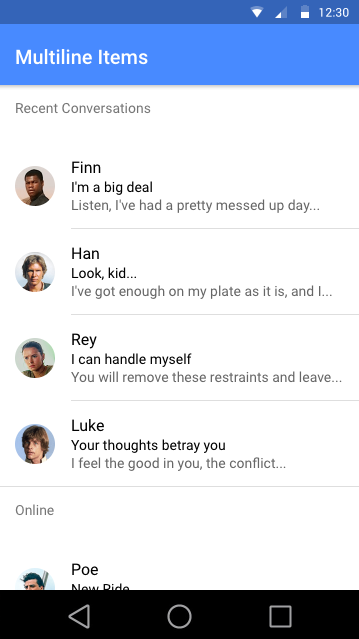
\includegraphics[scale=0.3,valign=t]{imagens/cmp1.png}
  }
  \subfloat[DateTime]{
    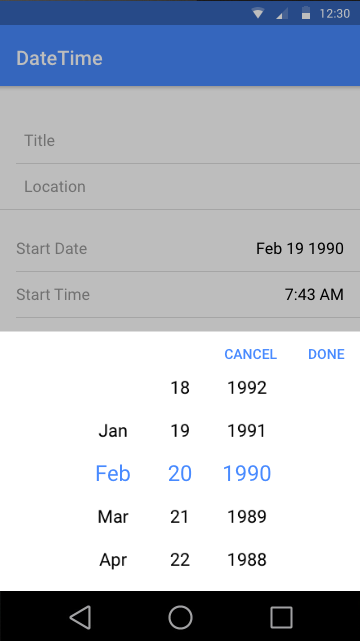
\includegraphics[scale=0.3,valign=t]{imagens/cmp2.png}
  }

  \subfloat[Float Action Buttons]{
    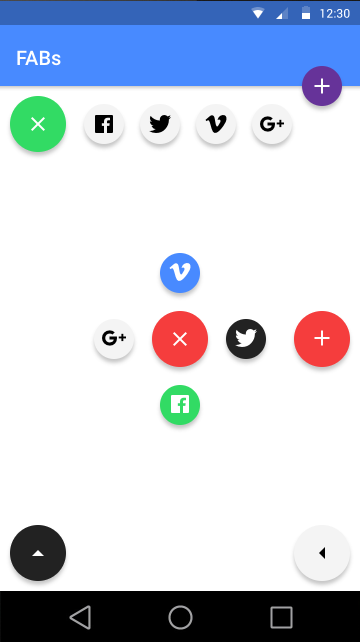
\includegraphics[scale=0.3,valign=t]{imagens/cmp3.png}
  }
  \subfloat[Menu]{
    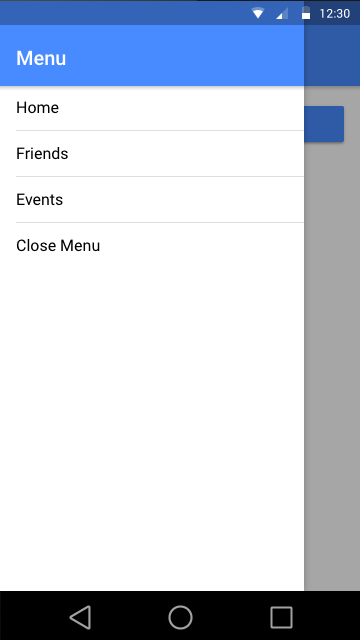
\includegraphics[scale=0.3,valign=t]{imagens/cmp4.png}
  }

  \subfloat[Checkboxes]{
    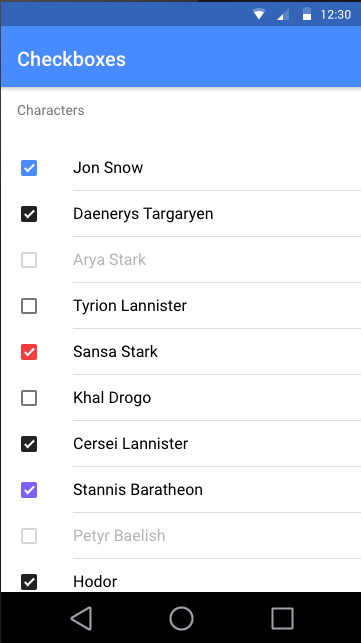
\includegraphics[scale=0.3,valign=t]{imagens/cmp5.png}
  }
  \subfloat[Action Sheets]{
    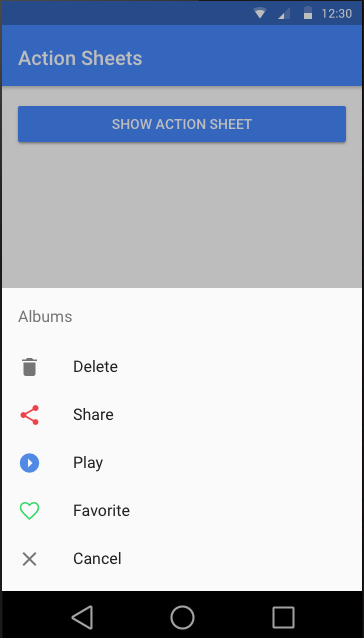
\includegraphics[scale=0.3,valign=t]{imagens/cmp6.png}
  }
  \caption{Exemplo de componentes no \textit{Ionic}}
  \label{fig:ionic_components}
\end{figure}

\subsection{Estrutura do Framework: \textit{FeathersJS}}

\textit{FeathersJS} é um \textit{framework} de código livre de desenvolvimento rápido para aplicações
web em tempo-real escritas em JavaScript. Disponibiliza uma arquitetura simples mas poderosa
para a construção de aplicações utilizando padrões de programação orientada a aspectos e serviços.
Os principais componentes do \textit{FeathersJS} são os \textit{services}, \textit{hooks} e
\textit{events} que são detalhados nas próximas seções.

\subsubsection{Services}

\textit{Services} ou serviços são a camada principal do \textit{\textit{FeathersJS}}.
Um serviço é simplesmente uma instância de uma classe JavaScript
que implementa métodos básicos para criação, consulta, atualização e
destruição de dados. Esse conjunto de operações ou funcionalidades é conhecido como
CRUD (\textit{Create, Read, Update, Delete}).

Os serviços no \textit{FeathersJS} expõem uma interface uniforme de acesso, permitindo
assim fornecer uma única API tanto para chamadas HTTP REST e \textit{websockets}.
Os verbos HTTP (GET, POST, PUT, PATCH e DELETE) têm a correspondência com
os métodos de um serviço no \textit{\textit{FeathersJS}} listados na \autoref{fig:service_interface}.

\begin{figure}[h]
\begin{lstlisting}[language=JavaScript]
const meuServico = {
  // GET /path
  find(params, callback) {},
  // GET /path/<id>
  get(id, params, callback) {},
  // POST /path
  create(data, params, callback) {},
  // PUT /path/<id>
  update(id, data, params, callback) {},
  // PATCH /path/<id>
  patch(id, data, params, callback) {},
  // DELETE /path/<id>
  remove(id, params, callback) {}
}
\end{lstlisting}
\caption{Interface de um serviço}
\label{fig:service_interface}
\end{figure}

\subsubsection{Hooks}

\textit{Hooks} são técnicamente \textit{middleware} ou funções que têm acesso aos
objetos de solicitação (\texttt{req}) e resposta (\texttt{res}).
Dessa forma os \textit{hooks} podem fazer mudanças nos objetos de solicitação e resposta.
O \textit{\textit{FeathersJS}} permite registrar \textit{hooks} antes (\textit{before}), depois
(\textit{after}) ou em caso de erro (\textit{error}) dos métodos de
um serviço, como mostrado na \autoref{fig:service_interface}.

Como eles têm acesso ao objetos de uma requisição (\texttt{req} e \texttt{res}), eles são usados
para política de controle de acesso da aplicação, registro de eventos, enviar
notificações, adicionar propriedades e muito mais.

Essa abordagem é conhecida como Programação Orientada a Aspectos (POA), que permite
a separação de propriedades ortogonais (ou que não fazem parte da funcionalidade
principal) dos componentes funcionais de uma forma natural e concisa.

Na \autoref{fig:hooks_example} três \textit{hooks} foram registrados para um serviço de questões (\textit{questions}) ($\ell.\,1$),
em que é adicionado a propriedade \texttt{createdAt} antes (\textit{before}) da criação (\textit{create}) de um objeto questão ($\ell.\,3-5$),
e a propriedade \texttt{updatedAt} quando uma questão é modificada (\textit{update} e \textit{patch}), ($\ell.\,7-13$).

\begin{figure}[h]
\begin{lstlisting}[language=JavaScript]
  app.service('questions').hooks({
    before: {
        create(hook) {
          hook.data.createdAt = new Date();
        },

        update(hook) {
          hook.data.updatedAt = new Date();
        },

        patch(hook) {
          hook.data.updatedAt = new Date();
        }
      }
  });
\end{lstlisting}
\caption{Exemplo registro de \textit{hooks} no \textit{\textit{FeathersJS}}}
\label{fig:hooks_example}
\end{figure}

\subsubsection{Events}

São os \textit{events} ou eventos no \textit{\textit{FeathersJS}} permitem
a criação de aplicações de tempo-real usando \textit{WebSockets}.

No \textit{\textit{FeathersJS}}, os serviços enviam automaticamente eventos ou notificações
\texttt{created, updated, patched, removed} quando algum dos respectivos métodos listados
na \autoref{fig:service_interface} finalizam com sucesso.
Os clientes da aplicação podem então ouvir a esses eventos e reagirem de acordo.

Na \autoref{fig:events_example} o cliente obtém uma referência do serviço
de votação ($\ell.\,2$) e então passa a ouvir quando uma nova votação é criada (\texttt{created}) ($\ell.\,5-7$).
Nesse caso, os clientes de uma aplicação de votação, por exemplo, poderiam
receber as questões da votação publicada por outro cliente e então responder.

\begin{figure}[h]
\begin{lstlisting}[language=JavaScript]
  // Retrieve the wrapped service object which will be an event emitter
  const poll = app.service('poll');

  // Listen `created` event
  poll.on('created', (poll) => {
    console.log('New poll created', poll);
  });
\end{lstlisting}
\caption{Exemplo eventos no \textit{\textit{FeathersJS}}}
\label{fig:events_example}
\end{figure}

\subsubsection{Visão geral}

A \autoref{fig:feathers_request} ilustra como funciona o ciclo de uma requisição
entre clientes e uma aplicação baseada no \textit{FeathersJS}.

O cliente faz uma requisição para um serviço, que antes de chegar no serviço passa
pela camada de \textit{before hooks}, o método requisitado pode completar com sucesso indo para a
\textit{after hooks} e enviando um evento para os clientes conectados. Qualquer erro no processo
é enviado para a camada \textit{error hooks} que também pode notificar os clientes da aplicação.

\begin{figure}
  \centering
  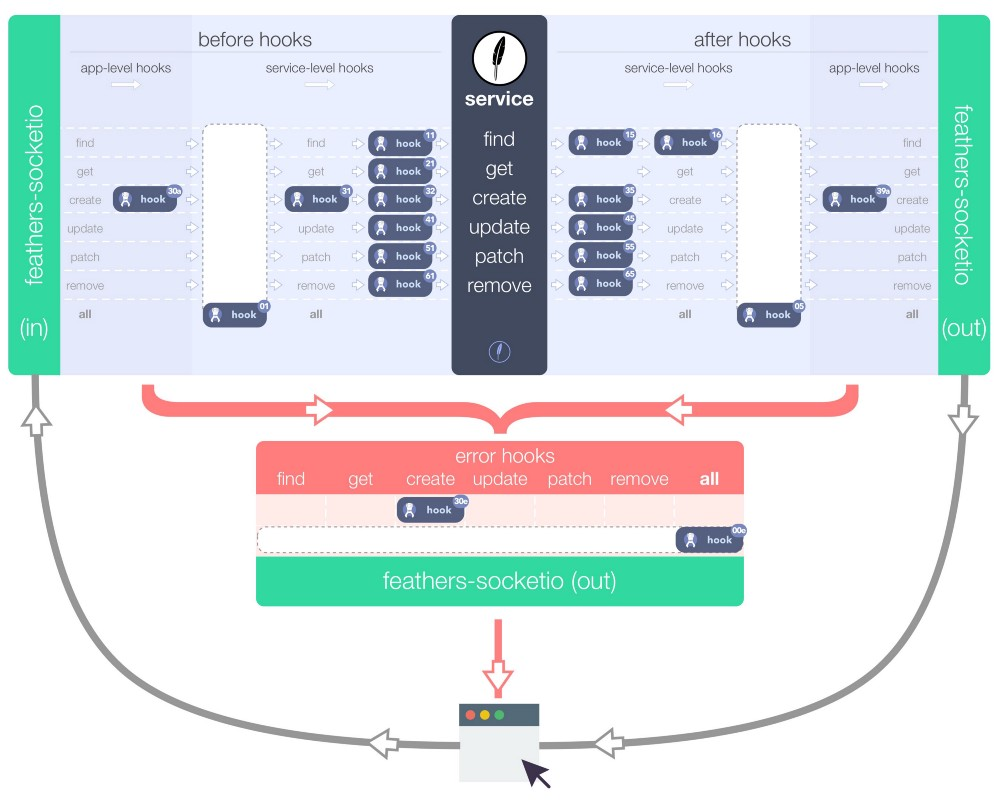
\includegraphics[scale=0.45,valign=t]{imagens/feathers_request.jpeg}
  \caption{Como o ciclo de uma requisição funciona no \textit{FeathersJS}}
  \label{fig:feathers_request}
\end{figure}

A utilização do \textit{FeathersJS} simplificou muito o processo de construção
do software por disponibilizar facilidades para o programador e implementar
uma API de tempo-real via serviços de forma nativa. Além disso, a interface dos
serviços \autoref{fig:service_interface} torna fácil a integração com qualquer banco de dados.
Nesse sentido, o \textit{FeathersJS} suporta alguns ORM que permitem uma integração
com uma variedade de banco de dados por meio de uma interface única.
